\makeatletter\let\ifGm@compatii\relax\makeatother
\documentclass[9pt,xcolor=pdftex,dvipsnames,table]{beamer}

\usepackage{amsmath}
\usepackage{multirow}
\usepackage{colortbl}
\usepackage{placeins}
\usetheme{Pittsburgh}

\usecolortheme[RGB={0,75,100}]{structure}
\useinnertheme{circles}

\definecolor{dragonflyblue}{RGB}{0,153,204}
\definecolor{cellyellow}{rgb}{0.988, 0.976, 0.545}
\definecolor{cellorange}{rgb}{0.988, 0.631, 0.357}
\definecolor{cellred}{rgb}{0.890, 0.318, 0.328}
\setbeamercolor{frametitle}{fg=white}
\setbeamertemplate{navigation symbols}{}

\newcommand\BackgroundPicture[2]{%
    \setbeamertemplate{background}{%
    \parbox[c][\paperheight]{\paperwidth}{%
 \includegraphics[width=#2\paperwidth]{#1}
         \hfill \vfill
      }}}

\newcommand\NoBackground{%
    \setbeamertemplate{background}{}
    }

\newenvironment{narrow}[2]{%
	\begin{list}{}{%
	\setlength{\topsep}{0pt}%
	\setlength{\leftmargin}{#1}%
	\setlength{\rightmargin}{#2}%
	\setlength{\listparindent}{\parindent}%
	\setlength{\itemindent}{\parindent}%
	\setlength{\parsep}{\parskip}}%
	\item[]}{\end{list}}

\usepackage{helvet}
\usepackage{mathptmx}
\usepackage{graphics}
\usepackage[english]{babel}
\usepackage{hhline}
\usepackage{booktabs}
\usepackage{array}
\usepackage{wrapfig}
\usepackage{tikz}

\title[Doing right research]{\textbf{-- From data to report --} \\ \vspace{0.15cm} State-of-the art tools for streamlining data management, analysis and report production in ecological research}
\author{Yvan Richard}

\institute[Dragonfly Science]
{
Dragonfly Science \\
Level 5, 158 Victoria St, Wellington \\
\medskip
{\emph{yvan@dragonfly.co.nz}}
}

\date[Vic]{6$^{th}$ August 2013}


\begin{document}
\BackgroundPicture{images/banner.png}{1.0}

\begin{frame}
\titlepage
\vspace{-1.5cm}
 \begin{center}
 \resizebox{!}{2cm}{
\includegraphics[width=1.2\textwidth]{images/damselfly.png}}
 \end{center}
 \vspace{-1.5cm}
\end{frame}


\begin{frame}{\textbf{Typical case \#1}}
\textbf{New data to be incorporated, or mistake in source data}
\begin{enumerate}
\item Add data to spreadsheet or correct mistake
\item Re-run analyses, involving thousands of clicks
\item Update figures, with a lot of frustration about formatting
\item Update tables, endless copy \& paste operations
\item Update numbers in report -- Have you missed one?
\end{enumerate}
\vspace{0.6cm}
Waste of time, stressful moment, ending up with a vague feeling of
having forgotten to update something...
\vspace{-0.5cm}
\end{frame}

\begin{frame}{\textbf{Typical case \#2}}
\textbf{Accidental deletion or bad direction}
\begin{itemize}
\item You realise at some stage that you deleted some data or some
  text a while ago and that you kept working in a wrong direction.
\item You wish you could go back in time to a previous version of your
  work
\item The deleted part might be lost forever, or at least requires to
  re-do everything since the mistake.
\end{itemize}
\vspace{0.6cm}
Waste of time and frustration! But you learn from your mistake, and
since then, you keep a different version of everything every time you
change something.
\vspace{-0.5cm}
\end{frame}

\begin{frame}{\textbf{Typical case \#3}}
\textbf{Coming back to an old project}
\begin{itemize}
\item The review of a submitted paper comes back and requires you to
  do additional analyses
\item You open your project folder only to discover 20-odd different
  versions of the data
\item Which one did you use?
\item After being fairly confident of the correct one to use, you
  re-do the analyses, and find different results!
\item Eventually, you manage by trial and error to find the same
  results and keep going.
\end{itemize}
\vspace{0.6cm}
Waste of time, ending up unsatisfied and not very confident about the results.
\vspace{-0.5cm}
\end{frame}


\begin{frame}{\textbf{Typical case \#4}}
\textbf{Changing computer}
\begin{itemize}
\item After spending a lot of time perfecting the formatting of your
  thesis, presentation, or article, you realise your document looks
  quite different on another computer
\end{itemize}
\vspace{0.6cm}
Panic and frustration...
\vspace{-0.5cm}
\end{frame}


\begin{frame}{\textbf{Typical case \#5}}
\textbf{Changing institution}
\begin{itemize}
\item After finally getting into grip with a given software, you
  change institution and you realise they use a different
  software. Unfortunately, you cannot get your favourite one because
  the license is too expensive.
\end{itemize}
\vspace{0.6cm}
Waste of time re-learning a new software, never becoming a master at a
given one
\vspace{-0.5cm}
\end{frame}


\begin{frame}{\textbf{Typical case \#6}}
\textbf{Auditing}
\begin{itemize}
\item You work on a sensitive issue, e.g. an endangered species at
  risk of a proposed development project.
\item The industry rejects your results, which prevent their project to
  be approved.
\item In the environmental court, it is agreed that your project gets
  audited, requiring you to show how got to these results step by step.
\end{itemize}
\vspace{0.6cm}
... Can you?
\vspace{-0.5cm}
\end{frame}



\begin{frame}{\textbf{Typical case \#7}}
\textbf{Teaching}
\begin{itemize}
\item A workmate or student asks you to show him/her how you do a
  certain analysis.
\item You sit at a computer with him/her, and start explaining: 
``You go to this menu, and click there, then there, then you go there
and type in that, and then you click on this, etc.''
\item It takes quite a while, as your workmate writes down the whole
  complicated process.
\item He/she gets back to you later, because his/her version of the
  program is slightly different and he/she cannot find a certain item
  in the menus.
\end{itemize}
\vspace{0.6cm}
... (sigh) ...
\vspace{-0.5cm}
\end{frame}


\begin{frame}{\textbf{Let's dream that...}}
\begin{itemize}
\item all these problems could be solved,
\item you could focus on content and process rather than formatting
  and eye-candy,
\item all the tools to solve these problems and do proper research are free,
\item on the way of solving these problems, you acquire great skills
  that would make you find a job very easily.
\end{itemize}
\vspace{0.6cm}
Well, yes, it is possible!
\vspace{-0.5cm}
\end{frame}


\begin{frame}{\textbf{Research}}
Research should:
\begin{itemize}
\item be reproducible
\item be transparent
\item have a functional work flow
\end{itemize}
\vspace{0.6cm}
Sounds trivial, but it is rarely the case!
\vspace{-0.5cm}
\end{frame}


\begin{frame}{\textbf{Open-source software}}
\begin{itemize}
\item Free!
\item Generally quite portable between operating systems
\item Huge community for support, bug checking and fixing, for new developments
\item Transparent with a non-restrictive license, allowing easy
  communications between programs.
\end{itemize}
\end{frame}


\begin{frame}{\textbf{Main functions}}
\begin{itemize}
\item Data preparation, exploration, analysis, and plotting
\item Reporting
\item Bibliography
\item Work flow
\item Version control
\item Distribution
\end{itemize}
\end{frame}


\begin{frame}{\textbf{Data preparation, exploration, analysis \\ and plotting}}
\begin{columns}
\column{0.4\textwidth}
\centering

\includegraphics[width=1\textwidth]{images/r-logo.png}
\column{0.6\textwidth}
\begin{itemize}
\item NZ product!
\item Software environment for statistical computing and graphics
\item Programming language, but easy to learn
\item Works on all systems (Windows, Mac, Linux, ...)
\item Increasing popularity, real threat to commercial products
  (e.g. SAS, SPSS)
\item Evolves fast, expandable with thousands of available packages
\end{itemize}
\end{columns}
\end{frame}


\begin{frame}[fragile] % Notice the [fragile] option beside \begin{frame} %
\frametitle{\textbf{R language}}
\begin{columns}
\column{0.5\textwidth}
\begin{example}[]
\begin{verbatim}
## Load data
dat <- read.csv("file-with-data.csv")

## Data manipulation
dat$var3 <- dat$var1 + dat$var2

## Plot
plot(var1, var2)
\end{verbatim} % Extra carriage return causes problem wit verbatim %
\end{example}
\column{0.48\textwidth}
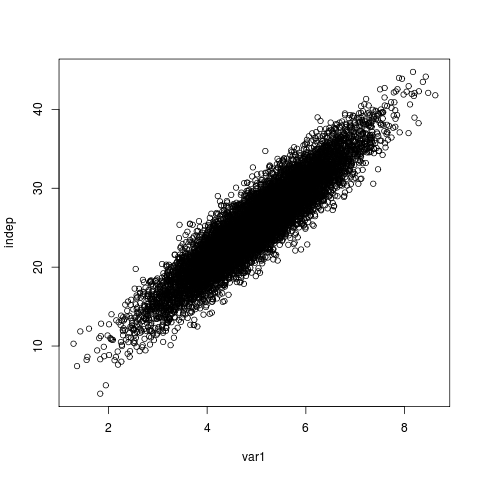
\includegraphics[width=1\textwidth]{images/corr.png}
\end{columns}
\end{frame}


\begin{frame}[fragile] % Notice the [fragile] option beside \begin{frame} %
\frametitle{\textbf{R language}}
Fitting a linear model
\begin{verbatim}
mod <- lm(dep ~ indep1 + indep2)
summary(mod)
\end{verbatim}

\scriptsize{
\begin{verbatim}
Call:
lm(formula = indep ~ var1 + var2)

Residuals:
    Min      1Q  Median      3Q     Max 
-7.8060 -1.3795 -0.0133  1.3950  8.2858 

Coefficients:
            Estimate Std. Error t value Pr(>|t|)    
(Intercept)  0.21056    0.23224   0.907   0.3646    
var1         4.95934    0.02074 239.112   <2e-16 ***
var2         0.04883    0.02062   2.368   0.0179 *  
---
Signif. codes:  0 ‘***’ 0.001 ‘**’ 0.01 ‘*’ 0.05 ‘.’ 0.1 ‘ ’ 1 

Residual standard error: 2.083 on 9997 degrees of freedom
Multiple R-squared: 0.8512,	Adjusted R-squared: 0.8511 
F-statistic: 2.859e+04 on 2 and 9997 DF,  p-value: < 2.2e-16
\end{verbatim} 
}
\end{frame}


\begin{frame}{\textbf{R: advanced graphics}}
\centering
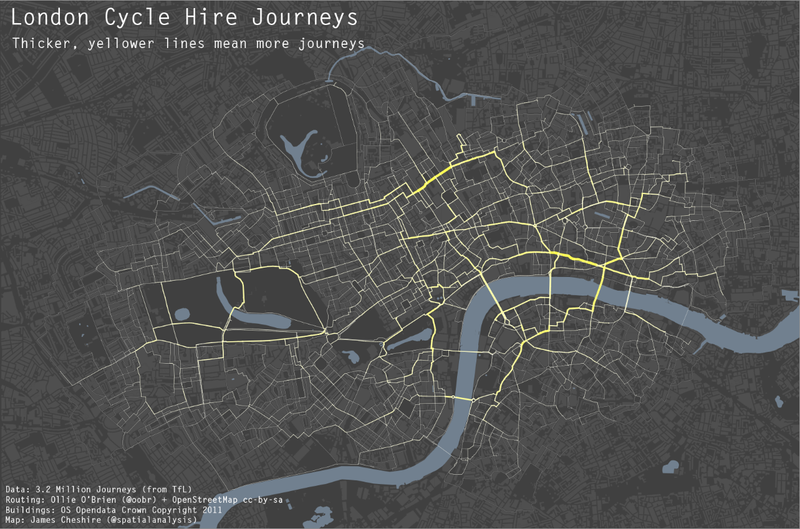
\includegraphics[width=1\textwidth]{images/bike-routes.png}
\vspace{-1cm}
\end{frame}

\begin{frame}{\textbf{Scripting power}}
  \begin{itemize}
  \item Everything is written, no lost clicks
  \item Reproducible
  \item Easily changed
  \item Code is re-usable
  \item Repetitive tasks are done using loops
  \item Generally quicker than clicks and navigating menus
  \end{itemize}
\end{frame}


\begin{frame}{\textbf{Reporting}}
\begin{columns}
\column{0.4\textwidth}
\centering

\includegraphics[width=1\textwidth]{images/LaTeX-logo.png}
\column{0.6\textwidth}
\begin{itemize}
\item Compiled documents, not WYSIWYG
\item Very common
\item Most scientific journals provide their own template
\item Beautiful typesetting
\item Takes care of formatting automatically
\item Maths formulae are easy to write
\item Easy PDF creation with pdflatex
\item Creation of presentations using Beamer (like this one)
\end{itemize}
\end{columns}
\end{frame}


\begin{frame}{\textbf{\LaTeX}}
\centering
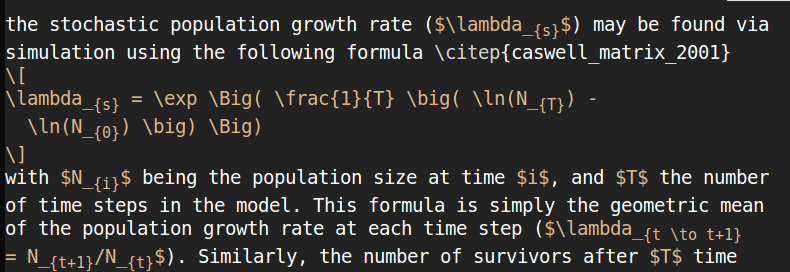
\includegraphics[width=.8\textwidth]{images/latex-ex.png} \\
\vspace{.5cm}
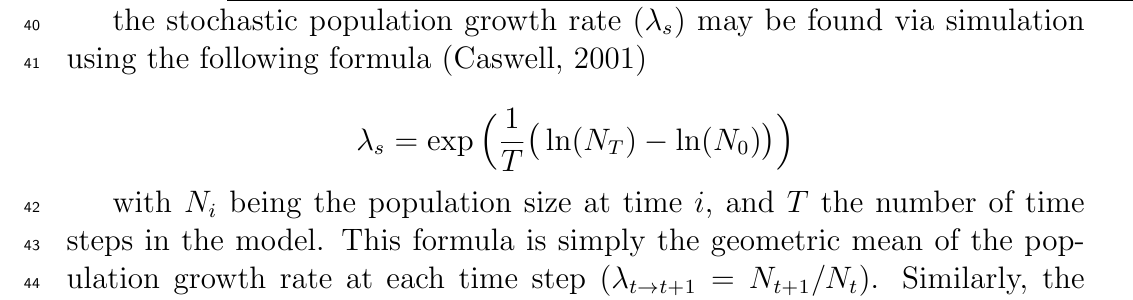
\includegraphics[width=1\textwidth]{images/latex-ex-pdf.png}
\end{frame}


\begin{frame}{\textbf{Calling R into LaTeX using Sweave}}
  \begin{itemize}
  \item Sweave lets data and tables from R to be included in LaTeX documents
  \item Why copying and pasting data manually when you can call them directly?
  \item Enormous time saver
  \item Chances of mistakes are minimal
  \item Initial data can be changed, the changes will be automatically
    reflected in the report 
  \end{itemize}
\end{frame}


\begin{frame}[fragile] 
\frametitle{\textbf{Calling R into LaTeX using Sweave}}
\begin{example}[]
\begin{verbatim}
\SweaveOpts{echo=FALSE, results=tex, prefix.string=sweave/fig}

<<load>>=
dat <- read.csv("file-with-data.csv")
minsize <- min(dat$popsize)
maxsize <- max(dat$popsize)
@ 

The population size varied between \Sexpr{minsize} and \Sexpr{maxsize}.
\end{verbatim}
\end{example}
\end{frame}


\begin{frame}[fragile]
\frametitle{\textbf{Bibliography in LaTeX}}
Including references is easy with BibTeX!
References are stored in a text file (e.g.: refs.bib):
\begin{verbatim}
@article{richard_cost_2010,
    title = "Cost distance modelling of landscape connectivity 
             and gap-crossing ability using radio-tracking data",
    volume = "47",
    number = "3",
    journal = "Journal of Applied Ecology",
    author = "Richard, Yvan and Armstrong, Doug P",
    year = "2010",
    pages = "603--610",
    },
\end{verbatim}
Then each reference is called in the LaTeX document by its tag:
\begin{verbatim}
... is a powerful tool to analyse movements \cite{richard_cost_2010}.
\end{verbatim}
\end{frame}


\begin{frame}{\textbf{Bibliography in \LaTeX}}
  \begin{itemize}
  \item BibTeX format is very common
  \item References in this format can be downloaded from Google
    Scholar, imported from Zotero, and from journals web site
  \item Templates exist for all journals
  \item No more corrupted EndNote databases...
  \end{itemize}
\end{frame}


\begin{frame}{\textbf{Workflow management}}
\begin{columns}
\column{0.4\textwidth}
\centering

\includegraphics[width=1\textwidth]{images/make-logo.jpg}
\column{0.6\textwidth}
  \begin{itemize}
  \item GNU make
  \item Centralise jobs to be run
  \item Jobs are run in order, and only if necessary
  \item Jobs can be run in parallel in order to use several computer processors
  \item Can be used to document the whole workflow.
  \end{itemize}
\end{columns}
\end{frame}


\begin{frame}[fragile] 
\frametitle{\textbf{Workflow management}}
The jobs are written in a text file (makefile):
\small{
\begin{verbatim}
all:  report.pdf

report.pdf:  report.tex datafile.csv refs.bib
    bibtex report 
    pdflatex report

datafile.csv:  analyse.r inputdata.csv
    Rscript analyse.r
\end{verbatim}}
\vspace{0.25cm}
You run the whole process by only typing ``make'' in a terminal, it's
that easy.
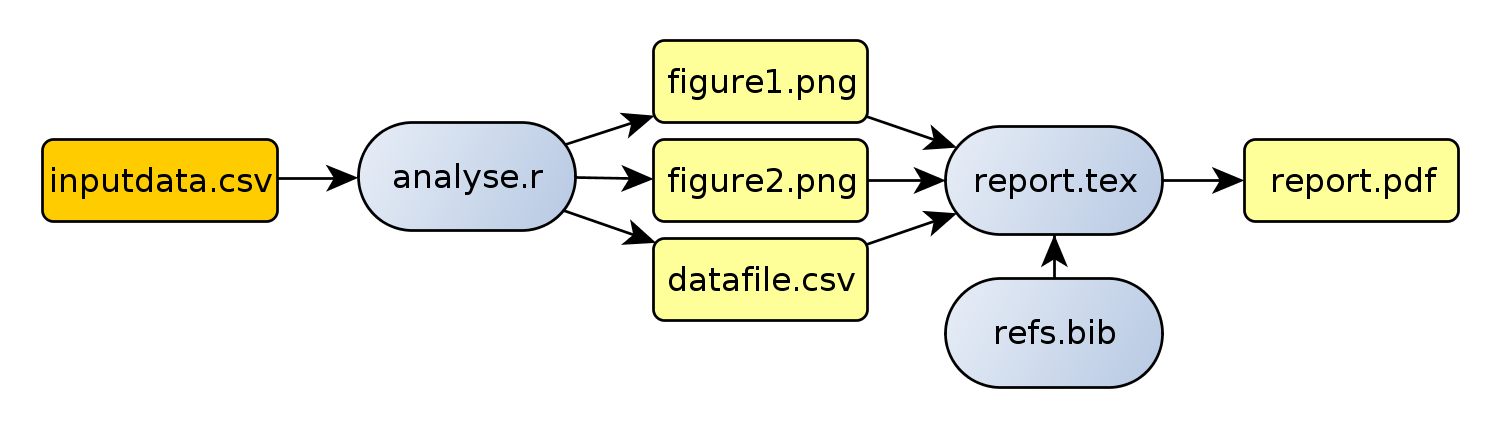
\includegraphics[width=1\textwidth]{images/workflow.png}
\vspace{-1cm}
\end{frame}


\begin{frame}{\textbf{Version control}}
\begin{columns}
\column{0.4\textwidth}
\centering

\includegraphics[width=1\textwidth]{images/git-logo.png}
\column{0.6\textwidth}
\begin{itemize}
\item Saves all gradual changes of files
\item Allows to safely keep only one version of each file 
\item Do not be afraid to delete stuff! You can always come back to previous versions
\item Provides an easy outlook of all modifications
\item Utilities to compare versions
\item Great also for cooperative work
\end{itemize}
\end{columns}
\end{frame}


\begin{frame}[fragile]
\frametitle{\textbf{Workflow management}}
Easy commands: \\
\verb=git status=: to get list of all modified files \\
\verb=git add .=: to inform git to save all modifications \\
\verb=git commit -m "Finished intro of chapter 3"=: to save locally the
current state of modifications, with a comment to describe the changes \\
\verb=git push=: to save the commits to the server
\end{frame}


\begin{frame}{\textbf{Distribution}}
\begin{columns}
\column{0.4\textwidth}
\centering

\includegraphics[width=1\textwidth]{images/github-logo.jpg}
\column{0.6\textwidth}
\begin{itemize}
\item GitHub is a web interface and service to store your git project
\item Makes it easy to access your project from anywhere and to share
  it with others
\item Free for open-source projects
\item Great for issue tracking (to-do list)
\end{itemize}
\end{columns}
\end{frame}



\begin{frame}{\textbf{Conclusions}}
\begin{itemize}
\item Great suite of tools for doing proper research, and they are all free!
\item Risk of mistakes minimised
\item Transparent and reproducible
\item Fun! Just like playing Lego
\item Adopting only one of these tools even is a great improvement
  over the traditional bad habits
\item This workflow allows tackling some large projects comfortably
  that would be impossible otherwise
\item These skills will help you all your life and make your life
  easier, and are great to get a job
\end{itemize}
But...
\begin{itemize}
\item It looks scary at first
\item Big learning curve
\end{itemize}
But still worth it 100\%!
\end{frame}


\end{document}

